\begin{figure*}[t]
\centering
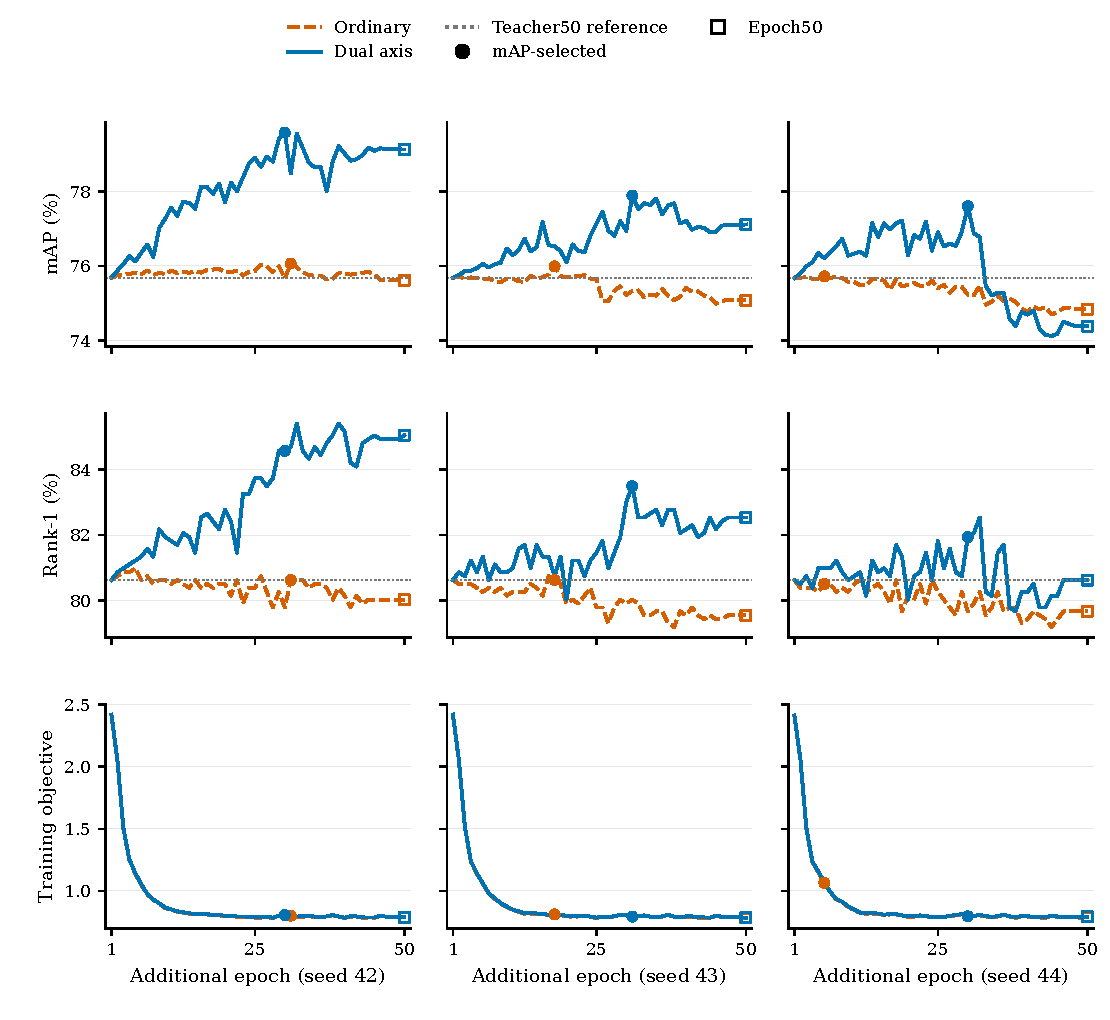
\includegraphics[width=0.95\textwidth]{expert_seed_curves.pdf}
\caption{RGBNT201 I training trajectories for three paired expert seeds42/43/44, conditional on the same frozen DeMo42 teacher. Ordinary and dual-axis arms each train an additional50 epochs with identical data, budgets and per-seed batch order. Dots mark each run's normal-mAP-selected checkpoint (also used on the Rank-1 and objective rows), open squares mark epoch50. The dotted DeMo line is the fixed50-epoch teacher reference, not an equal-total-budget trained arm. Full official benchmark selected epochs; no untouched-test or whole-pipeline variance claim. Axis seed44 loses3.226686 mAP points after its selected peak; all runs and negative trajectories remain visible.}
\label{fig:expert-seed-curves}
\end{figure*}

\begin{figure*}[t]
\centering
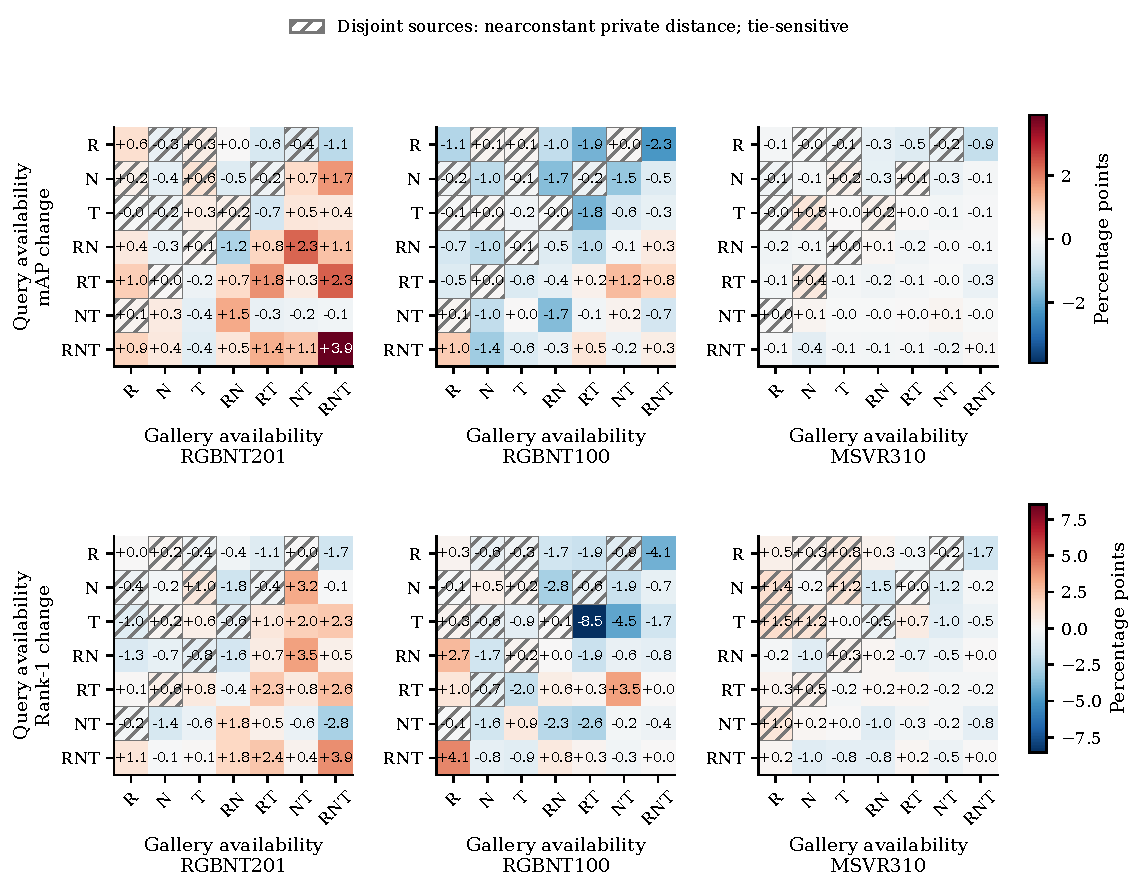
\includegraphics[width=0.95\textwidth]{fixed_best_missing49.pdf}
\caption{I42 dual-axis full11 minus its own availability-aware frozen base00 in each of49 query/gallery modality combinations, on the three complete official query/gallery datasets. Values are percentage-point changes; one fixed normal-mAP-selected checkpoint per dataset, never selected by missing condition. All49 include the full-input cell; cells are correlated repeated-query diagnostics, not independent replicates or pooled mAP. Hatching marks the12 source-disjoint combinations: private coordinates have nearconstant distance2, so numerical/tie changes do not establish cross-source identity retrieval. R/N/T denote RGB/NIR/TIR. Separate zero-centered metric color scales are shared across all datasets.}
\label{fig:fixed-best-missing49}
\end{figure*}
